\input ../SlidePreamble
\input ../preamble


\begin{document}

{\Huge

  \centerline{\bf TTIC 31230, Fundamentals of Deep Learning}
  \bigskip
  \centerline{David McAllester, Autumn 2022}
  \vfill
  \vfil
  \centerline{Improving Diffusion Models}
  \vfill
  \vfill

\slidetwo{Improved Denoising Diffusion Probabilistic Models}
{Nichol and Dhariwal, February 2021}

We can compare any two models of a distribution by computing upper bounds on cross-entropy loss for each model.

\vfill
Since gradient descent on corss entropy (GPT-3) is so successful, maybe we shuld also be doing {\bf graduate student descent} on cross entropy.

\vfill
In other words, cross entropy may be an undervalued metric for comparing different systems trained with different architectures.


\slide{Improved Cross-Entropy Loss}

For image models the cross entropy is generally refered to as negative log likelihood (or NLL) and is measured in bits per image channel.

\centerline{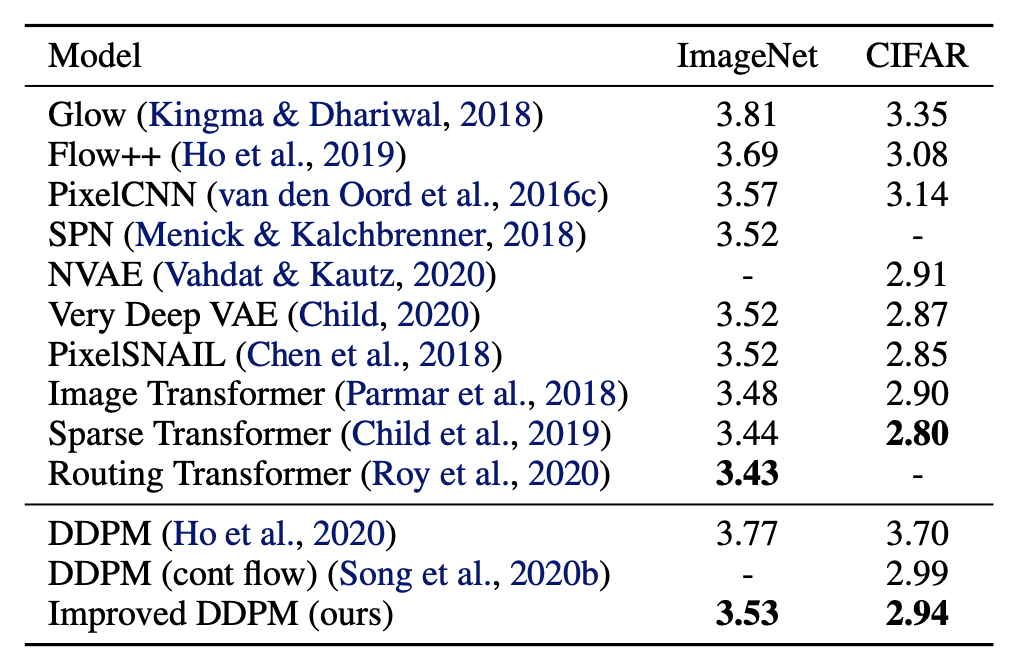
\includegraphics[width=5in]{\images/DiffNLL}}

\slide{Reducing the variance of the VLB}

The community seems to be now calling the ELBO the VLB (variational lower bound).  Perhaps a slight to Bayesians.

\vfill
For a progressive VAE with layers $z_0,\ldots,z_L$ where $z_0 = y$ the VLB (ELBO) gives

{\huge
\begin{eqnarray*}
- \ln p_{\gen}(z_0) & \leq & E_\enc\; -\ln \frac{p_\gen(z_L,\ldots,z_0)}{p_\enc(z_1,\ldots,z_L|z_0)}
\\
\\
\\
& = & E_\enc -\ln p_\pri(z_L) - \sum_{\ell } \frac{\ln p_\dec(z_{\ell-1}|z_\ell)}{\ln p_\enc(z_\ell|z_{\ell-1})}
\end{eqnarray*}
}

\slide{Reducing the variance of the VLB}

{\huge
\begin{eqnarray*}
- \ln p_{\gen}(z_0) & \leq & E_\enc\; -\ln \frac{p_\gen(z_L,\ldots,z_0)}{p_\enc(z_1,\ldots,z_L|z_0)}
\\
\\
\\
& = & E_\enc -\ln p_\pri(z_L) - \sum_{\ell } \frac{\ln p_\dec(z_{\ell-1}|z_\ell)}{\ln p_\enc(z_\ell|z_{\ell-1})}
\end{eqnarray*}
}

\vfill
For a diffusion model this expression can be converted into a form involving KL divergences between Gaussians which can be calculated analytically.

\slide{Measuing Cross Entropy}

{\huge
\begin{eqnarray*}
- \ln p_{\gen}(z_0) & \leq & E_\enc -\ln p_\pri(z_L) - \sum_{\ell } \ln \frac{p_\dec(z_{\ell-1}|z_\ell)}{p_\enc(z_\ell|z_{\ell-1})} \\
\\
& = & E_\enc -\ln p_\pri(z_L) - \sum_{\ell } \ln \frac{p_\dec(z_{\ell-1}|z_\ell)}{p_\enc(z_\ell|z_{\ell-1},z_0)} \\
\\
& = & E_\enc -\ln p_\pri(z_L) - \sum_{\ell } \ln \frac{p_\dec(z_{\ell-1}|z_\ell)p(z_{\ell-1}|z_0)}{p_\enc(z_\ell,z_{\ell-1}|z_0)} \\
\\
& = & E_\enc -\ln p_\pri(z_L) - \sum_{\ell } \ln \frac{p_\dec(z_{\ell-1}|z_\ell)p_\enc(z_{\ell-1}|z_0)}{p_\enc(z_{\ell-1}|z_\ell,z_0)p_\enc(z_\ell|z_0)}
\end{eqnarray*}
}


\slide{Measuring The Cross Entropy}

{\huge
\begin{eqnarray*}
- \ln p_\gen(z_0) & \leq & E_\enc -\ln p_\pri(z_L) - \sum_{\ell } \ln \frac{p_\dec(z_{\ell-1}|z_\ell)}{p_\enc(z_{\ell-1}|z_\ell,z_0)}
- \ln \frac{p_\dec(z_{\ell-1}|z_0)}{p_\enc(z_\ell|z_0)} \\
\\
& = & E_\enc -\ln \frac{p_\pri(z_L)}{p_\enc(z_L|z_0)} - \sum_{\color{red} \ell \geq 2} \ln \frac{p_\dec(z_{\ell-1}|z_\ell)}{p_\enc(z_{\ell-1}|z_\ell,z_0)} - \ln p_\dec(z_0|z_1) \\
\\
\\
& = & E_\enc \left\{\begin{array}{l}KL(p_\pri(z_L),p_\enc(z_L|z_0)) \\
\\
+ \sum_{\ell \geq 2} KL(p_\dec(z_{\ell-1}|z_\ell),p_\enc(z_{\ell-1}|z_\ell,z_0)) \\
\\
- \ln p_\dec(z_0|z_1) \end{array} \right.
\end{eqnarray*}
}


\slide{Measuring The Cross Entropy}

{\huge
\begin{eqnarray*}
- \ln p_\gen(z_0) & \leq &
E_\enc \left\{\begin{array}{l}KL(p_\pri(z_L),p_\enc(z_L|z_0)) \\
\\
+ \sum_{\ell > 1} KL(p_\dec(z_{\ell-1}|z_\ell),p_\enc(z_{\ell-1}|z_\ell,z_0)) \\
\\
- \ln p_\dec(z_0|z_1) \end{array} \right.
\end{eqnarray*}
}

All of the KL-divergences can be computed analytically from Gaussians.  This reduces the variance in estimating the bound.

\vfill
Nichol and Dhariwal compute $- \ln p_\dec(z_0|z_1)$ by treating each image channel as a discrete set of 256 values and computing the probability that a draw from
the computed Gaussian rounds to the actual discrete value.

\slide{Optimizing the Decoder Variances}

$$\dec(z_\ell,\ell) = \frac{1}{\sqrt{1-\sigma_\ell^2}}\left(z_\ell - \sigma_\ell\; \epsilon(z_\ell,\ell)\right)\; +\; \tilde{\sigma}_\ell\delta\;\;\;\;\;\delta \sim {\cal N}(0,I)$$

\vfill
Nichol and Dhariwal train the decoder noise $\tilde{\sigma}_\ell$ with the VLB objective.

\vfill
This significantly improves the value of the VLB (not surprising).

\slide{Optimizing the Decoder Variances}

$$\dec(z_\ell,\ell) = \frac{1}{\sqrt{1-\sigma_\ell^2}}\left(z_\ell - \sigma_\ell\; \epsilon(z_\ell,\ell)\right)\; +\; \tilde{\sigma}_\ell\delta\;\;\;\;\;\delta \sim {\cal N}(0,I)$$

\vfill
Training $\tilde{\sigma}_\ell$ by optimizing the VLB gives $\tilde{\sigma}_\ell < \sigma_\ell$ which makes the decoder more deterministic.

\vfill
We can think of $\tilde{\sigma}_\ell$ as secifying the numerical precision of the decoder output.

\vfill
Making the decoder more deterministic (higher precision) reduces the required number of levels from 1000 to 50 while still achieving good cross entropy loss.

\slide{Optimizing the Decoder Variances}

Song, Meng and Ermon, October 2021, found independently that deterministic decoding allows the number of levels to be reduced while achieving similar FID scores.

\vfill
The deterministic decoding version is called DDIM (denoising diffusion implicit models) as opposed to the original version DDPM
(denoising diffusion probabilistic models).

\vfill
But decoding over infinite precision reals destroys the VLB.

\slidetwo{Diffusion Models Beat GANs on Image Synthesis}{Dharwali and Nichol, May 2021}

\centerline{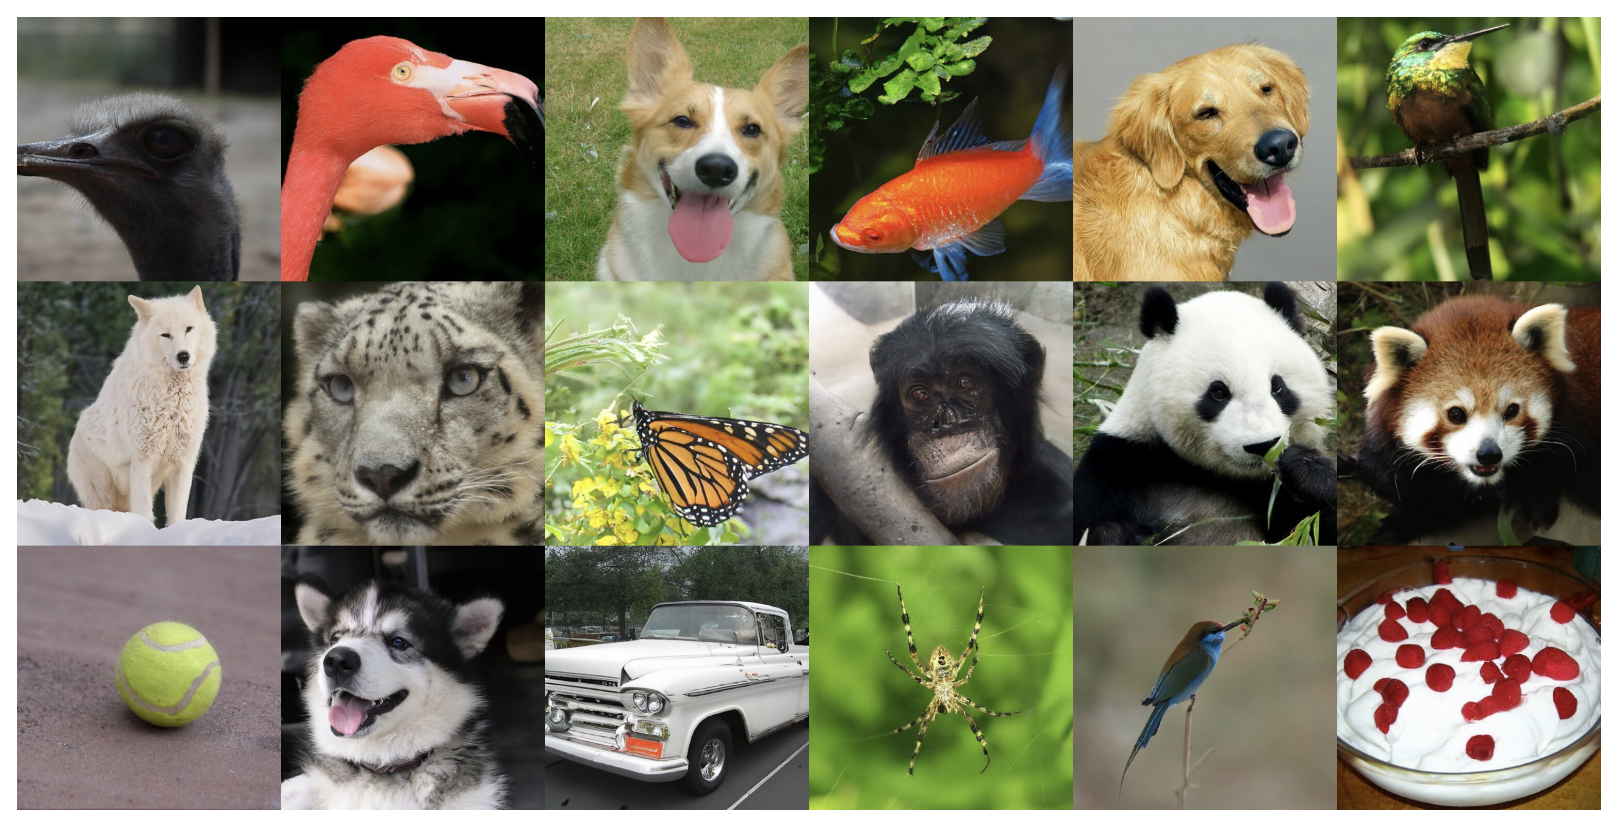
\includegraphics[width = 6in]{\images/DiffGAN}}

\slide{Class-Conditional Generation}

Consider training a model $\Phi$ on pairs $(x,y)$ using

$$\Phi^* = \argmin_\Phi\;-\ln\;P_\Phi(y|x)$$

\vfill
We are interested in the case where $y$ is an image or sound wave and we consider sampling $y$ from $P_\Phi(y|x)$.

\vfill
Here we consider the case where $x$ is a class label (as in a class conditional GAN).

\vfill
We assume that we can train a model of $P(x|y)$  --- for example an ImageNet classifier.

\slide{Class-Conditional Generation}

$$\Phi^* = \argmin_\Phi\;-\ln\;P_\Phi(y|x)$$

\vfill
We assume a model of $P(x|y)$.

\vfill
Sampling $y$ from $P_\Phi(y|x)$ can be done by sampling the pair $(y,x)$ from a the joint distribution defined by $p_\Phi(y)P(x|y)$.

\slide{Using the Score Matching (thermodynamic) Interpretation}

Compare the decoding update
$$z_{\ell-1} = \frac{1}{\sqrt{1-\sigma_\ell^2}}\left(z_\ell - \sigma_\ell\; \epsilon(z_\ell,\ell) \right)\; +\; \tilde{\sigma}_\ell\delta$$

\vfill
with the thermodynamic interpretation

$$z_{t+1} = z_t + \nabla_z \;\score(z) + \sigma \delta$$


\slide{Using the Score Matching (thermodynamic) Interpretation}
\begin{eqnarray*}
  z_{\ell-1} & = & \frac{1}{\sqrt{1-\sigma_\ell^2}}\left(z_\ell - \sigma_\ell\; \epsilon(z_\ell,\ell) \right)\; +\; \tilde{\sigma}_\ell\delta \\
  \\
  z_{t+1} & = & z_t + \nabla_z\; \score(z) + \sigma \delta
\end{eqnarray*}


\vfill
Ignoring the expansion term we get that $- \sigma_\ell \epsilon(z_\ell,\ell)$ is identitified with $\nabla_z\; \score(z)$.

\slide{Using the Score Matching (thermodynamic) Interpretation}
\begin{eqnarray*}
  z_{\ell-1} & = & \frac{1}{\sqrt{1-\sigma_\ell^2}}\left(z_\ell - \sigma_\ell\; \epsilon(z_\ell,\ell) \right)\; +\; \tilde{\sigma}_\ell\delta \\
  \\
  z_{t+1} & = & z_t + \nabla_z\; \score(z) + \sigma \delta
\end{eqnarray*}


\vfill

\vfill
Taking $\score(z,x) = \score(z) + \ln P(x|z)$, and introducing a hyperparameter $s$, we can do an update on the joint score as


$$\dec(z_\ell,\ell) = \frac{1}{\sqrt{1-\sigma_\ell^2}}\left(z_\ell - \sigma_\ell\; \epsilon(z_\ell,\ell) + {\color{red} s \nabla_{z} \ln P(x|z)}\right)\; +\; \tilde{\sigma}_\ell\delta$$


\slide{Using the Score Matching (thermodynamic) Interpretation}

$$\dec(z_\ell,\ell) = \frac{1}{\sqrt{1-\sigma_\ell^2}}\left(z_\ell - \sigma_\ell\; \epsilon(z_\ell,\ell) + {\color{red} s \nabla_{z} \ln P(x|z)}\right)\; +\; \tilde{\sigma}_\ell\delta$$

\vfill
Empirically it was found that $s > 1$ is needed to get good class specificity of the generated image.

\slide{Other Improvements}

Various architectural choices in the U-Net were optimized based on FID score (not NLL).

\slide{Voila: Class-Conditional Image Generation}

\centerline{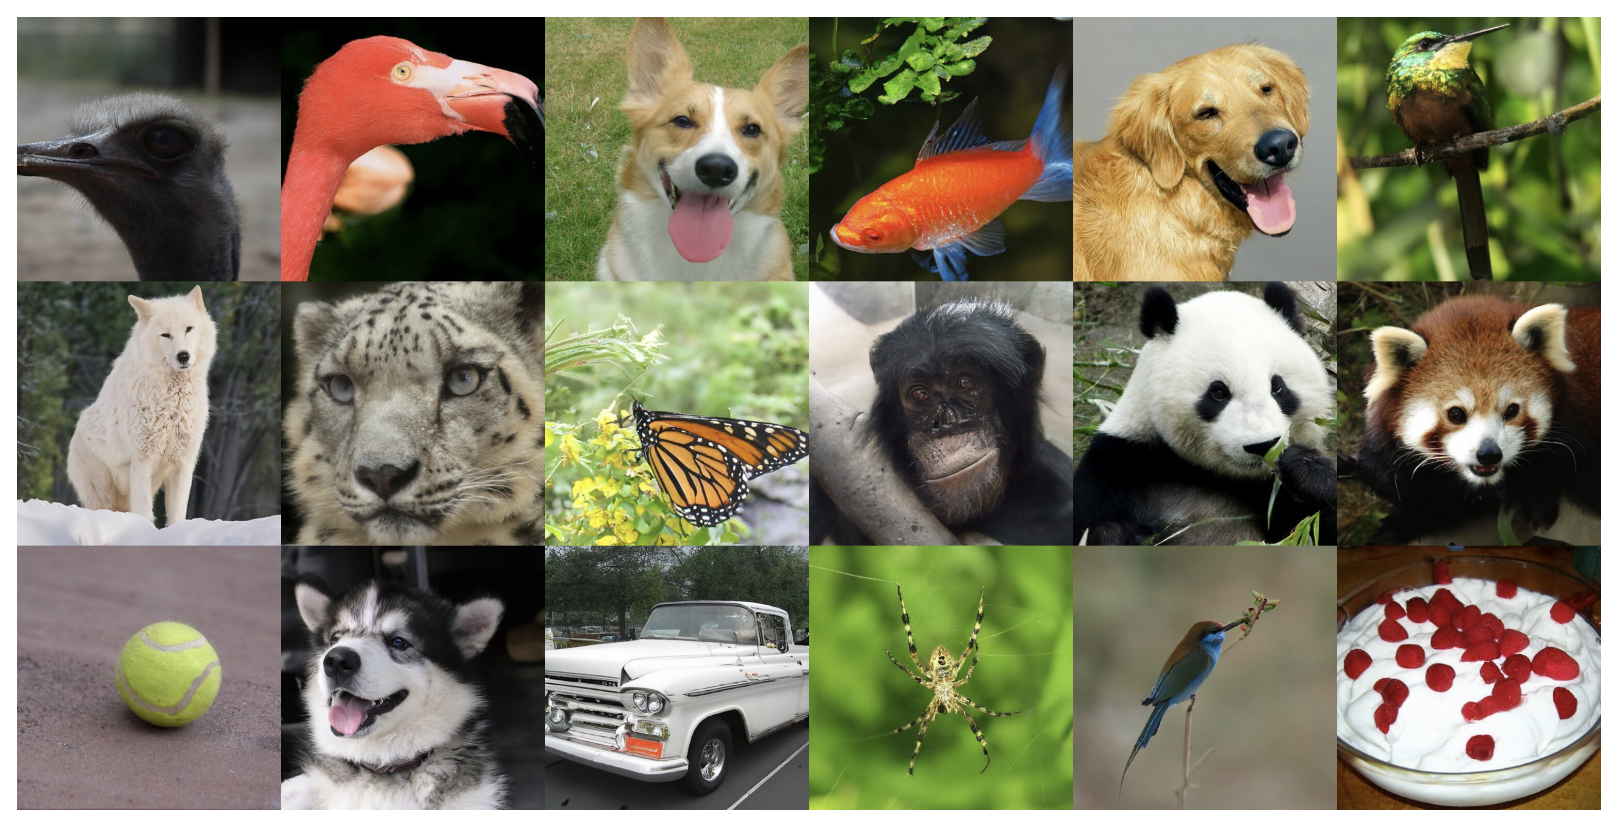
\includegraphics[width = 6in]{\images/DiffGAN}}

\slidetwo{Classifier-Free Diffusion Guidance}
{Ho and Salimans, December 2021 (NeurIPS workshop)}

We assume training data consisting of $(x,y)$ pairs.

\vfill
An obvious approach to conditional diffusion models $P(y|x)$ is to draw a pair $(x,y)$ and pass the conditioning information $x$ to the decoder
$\epsilon(z_\ell,\ell,x)$ when decoding for $z_0 = y$.

\vfill
This simple modification to the decoder seems to be insufficient (no one is using the naive approach).

\vfill
Instead people have modified the naive approach by modeling $P(x|z)$ in terms of the conditional decoder.

\slide{Classifier-Free Diffusion Guidance}

As in the naive approach we pass the conditional information to the decoder and train $\epsilon(z_\ell,\ell,x)$ to generate the $y$ associated with $x$.

\vfill
But 5\% of the time we set $x = \emptyset$ where $\emptyset$ is a fixed value unrelated to the image.

\vfill
We then interpret generation conditioned on $\emptyset$ to model the marginal distribution on $y$.

\slide{Classifier-Free Diffusion Guidance}

We now observe
$$p(x|y) = \frac{p(y|x)p(x)}{p(y)} \propto \frac{p(y|x)}{p(y)}$$

\vfill
This allows to take $\score(x|y) = \score(y|x) - \score(y)$.

\vfill
Following the thermodynamic interpretation we interpret $- \epsilon(z_\ell,\ell,x)$ as $\nabla_z\; \score(z_\ell|x)$

\vfill
This gives

$$\nabla_z \ln P(x|z) = \epsilon(z_\ell,\ell,\emptyset) - \epsilon(z_\ell,\ell,x)$$


\slide{Classifier-Free Diffusion Guidance}

The classifier-guided decoding
$$\dec(z_\ell,\ell) = \frac{1}{\sqrt{1-\sigma_\ell^2}}\left(
\begin{array}{l}z_\ell - \sigma_\ell \epsilon(z_\ell,\ell) \\
  {\color{red} +  \; s \nabla_{z} \ln P(x|z)}\end{array}\right)\; +\; \tilde{\sigma}_\ell\delta$$

can be written as
$$\dec(z_\ell,\ell) = \frac{1}{\sqrt{1-\sigma_\ell^2}}\left(z_\ell - \sigma_\ell {\color{red} \hat{\epsilon}(z_\ell,\ell)}\right)\; +\; \tilde{\sigma}_\ell\delta$$

with
$${\color{red} \hat{\epsilon}(z_\ell,\ell)} = \epsilon(z_\ell,\ell) - s'\nabla_z \ln P(x|z)$$

\slide{Classifier-Free Diffusion Guidance}
$$\hat{\epsilon}(z_\ell,\ell) = \epsilon(z_\ell,\ell) - s'\nabla_z \ln P(x|z)$$

$$\nabla_z \ln P(x|z) = \epsilon(z_\ell,\ell,\emptyset) - \epsilon(z_\ell,\ell,x)$$

gives

$$\hat{\epsilon}(z_\ell,\ell) = \epsilon(z_\ell,\ell,\emptyset) - s'(\epsilon(z_\ell,\ell,\emptyset) - \epsilon(z_\ell,\ell,x))$$

\vfill
where we take $s' > 1$ so that we are repelled from $\epsilon(z_\ell,\ell,\emptyset)$

\slide{Classifier-Free Diffusion Guidance}

$$\hat{\epsilon}(z_\ell,\ell) = \epsilon(z_\ell,\ell,\emptyset) - s'(\epsilon(z_\ell,\ell,\emptyset) - \epsilon(z_\ell,\ell,x))$$

\vfill
I am not convinced by this derivation but the result is intuitive --- drive away from images in general and toward the conditioned distribution to increase the effect of the conditioning.

\vfill
It seems likely to me that this hurts NLL while strengthening use of the condition information.

\slidetwo{GLIDE: Towards Photorealistic Image Generation ...}
         {Nichol, Dhariwal, Ramesh, et al., March 2022}

Slides under development.


\slide{END}
}
\end{document}
